\documentclass{article}
\usepackage{natbib}
\usepackage{graphicx}
\usepackage{amsmath}
\usepackage{hyperref}
\hypersetup{
colorlinks=false,
pdfborder={0 0 0},
}
\bibliographystyle{apalike}
\title{Research proposal}
\author{Mateusz Dadej}
\date{\today}

\begin{document}

\maketitle
As the 2008 financial crisis has shown, the interbank connections played a crucial role in propagating the financial contagion (\citet{bruner}). That is why a lot of attention has been paid since 2008 to analyze how the network structure of banks affects the contagion dynamics during crises. A seminal work from \citet{gai} shows with a simple model how the financial systems exhibit a tendency to be "robust-yet-fragile", that is while the probability of contagion may be low, the effects can be extremely widespread
when problems occur. Their model simulates a random network of interbank linkages with a shock to one of the banks. Based on similar model \citet{elliot} shows that diversification (more links per bank) connects the network initially, permitting cascades to travel; but as it increases further, organizations are better insured against one another's failures. Both of these studies analyze the contagion through insolency, that is a default of a single bank induces a loss to its borrowers, that may in turn default as well if their capital is insufficient. \citet{Greenwood} and \citet{cifuentes} models another contagion through fire sales and common exposure, where sudden sales of an asset reduces its price and thus impact the balance sheet of other banks with mark-to-market valuations.

However, much of the literature models assumes an exogenous formation of networks and often a passive reaction of the agents to the changing environment and as \citet{elliot} noted, "A fully endogenous study
of the network of cross-holdings and of asset holdings is a natural next step". This is the aim of research done in \cite{halaj}, where a model of banks form a network of interbank connections by optimizing their portfolio for assets and liabilites for better risk adjusted return. In their agent based model, the banks are first deciding their optimal asset and liability structure and then negotiate between each other the volume of interbank deposits and loans in a bargainig game. \citet{wolski} expande the model described in \citet{halaj} to secured and unsecured interbank loans and examine the effects of unconventional monetary policy on financial stability. In their model, the banks are using two different strategies to form forecasts of the risk premium that's later used to allocate resources to 4 different classes (bonds, long-term projects, secured and unsecured interbank loans). During trading, the bank that offers the highest rate and asks for lowest are matched, thus the process is similar to trading in any other part of financial market. The parameters are set either to be as the aggregate statistics (e.g. bonds yield is equal to average yield on German bund) or discretionally by the authors. In a banking model of \citet{aldasoro}, the agents are determining price on the interbank market through tâtonnement process. Their model can replicate real-world features of interbank model, that is core-periphery structure, low density and dis-assortative behavior. By showing varying model parameters, the study shows the systematic risk under various policy scenarios (changes to regulatory requirements) and role of different channels of systematic risk (liquidity hoarding, interconnections and fire sales). Similarily, \citet{liu}, uses data from financial statements of US banks, to parametrize an agent based model with endogenous networks. They show that had the 2008 crisis happen during 2017, the banking sector would experience less severe damage. \citet{NBERw29467} shows with an analytical model (unlike previously mentioned ABMs), how banks by optimizing their financial decisions endogenously lead to formation of the so called "core-periphery network". According to empirical literature (see e.g. \citet{intveld}), this kind of network structure is exhibited by interbank market. \citet{calimani} extend standard ABMs with asset managers to study fire sales dynamics with endogenous price formations. They show that asset managers absorb small liquidity shocks, but they exacerbate contagion when their voluntary liquid buffers are fully utilized.

I believe this is an interesting direction of future research. The way financial institutions price the assets and liabilites that are forming networks between them. And as the contagion dynamic changes how are they responding. The more specific research would perhaps extend current models by endogenously modeling equity cross-holdings or evaluating specific policy scenario with such model. 

\subsection*{Simple model of contagion with endogenous network}

In order to exhibit how endogenous networks form, this section will present a simple model based on \citet{gai}, with exogenous networks and then I will extend it with endogenously formed ones. The purpose of this section is to present the high-level overview of the endogeneity of the networks and its role in dynamics of financial contagion.

Each of $n$ banks has a balance sheet that is composed of interbank loans $A^{ib}_i$, external assets $A^{M}_i$ (e.g. mortgages) and on the liability side, interbank liabilities $L^{ib}_i$, client deposits $D_i$ and capital $K_i$. Every interbank asset is another bank's interbank liability, thus the claims form a network. The standard balance sheet identity holds:

$$A^{M}_i + A^{ib}_i = L^{ib}_i + D_i + K_i$$

Whenever capital is negative, the particular bank is considered insolvent. As the model assumes $0\%$ recovery rate, every interbank loan loses its value. Consequently, the creditors are under risk of further insolvency that can materialize if the level of capital is insufficient. This can further create a contagion in the system. 

To reproduce the main results from \citet{gai}, the interbank network of claims of 1000 banks was randomly generated with na Erdős–Rényi graph (each node has a given number of expected links). With few exceptions: 1) banks cannot lend to each other, 2) each bank needs to have at least one asset. The capital rate ($\frac{K_i}{A^{M}_i + A^{ib}_i}$) is set to $4\%$ and the amount of external and interbank assets to respectively 80 and 20 (the total assets are spread equally through every interbank loan). 

A contagion simulation is run with a single randomly chosen bank declaring default. Then each insolvent bank is defaulting on its debt firther spreading iteratively the contagion until there is no change in number of defaults. The system contagion is considered only after at least 5\% of every bank defaulted. To assess the asymptotic properties of the model was run 100 times for different number of probability of connection (or in other words number of interbank links). The figure 1 replicates the main findings of the \citet{gai}. The X axis shows the probability $p$ for each of the bank banks to have a link with each other, thus the average degree of the bank is approximately equal $p \times n$ where $n = 1000$. 

\begin{figure}[h]
    \centering
    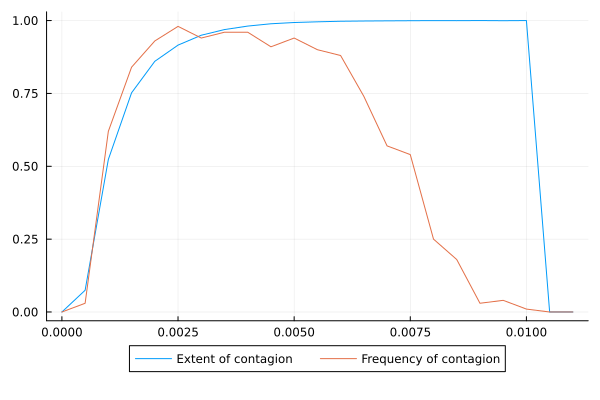
\includegraphics[scale=0.6]{contagionplot.png}
    \caption{contagion for different degree of the network}
\end{figure}

The figure shows the so called "robust-yet-fragile" tendency of banking system. At first when the banks diversify their interbank connections from 0 to 0.0025 because the interbank assets allow contagion to spread both the frequency (or probability of) system contagion is increasing. Then, the frequency of system contagion is decreasing with higher average degree but whenever it occures, the damage of is more severe as almost every bank defaults. There is a tipping point for the system when average degree of the network is high enough, the frequency of system contagion is close to 0.

Now we can extend the above model where given amount of interbank loan demand $\Delta_i$ and cash $C_i$ of each bank the system is solving an optimization problem to match the funds. An issue of this setting is that the whole system is solving a single optimization problem, whereas to better reflect the reality each bank should solve his own. At the same time this should be close enough for the purpose of herein section. The optimization problem is following:

\begin{equation}
    \begin{aligned}
    \min_{A^{ib}_i} \quad & (A^{ib}_i)^T A^{ib}_i - \gamma \cdot \left((A^{ib}_i)^T \frac{1}{k_i}\right)\\
    \textrm{s.t.} \quad & A^{ib}_{i,i} = 0 & \forall \; i \in N\\
      & A^{ib}_i \geq 0 & \forall \; i \in N\\
      & \sum_i^n A^{ib}_i \leq \Delta_i & \forall \; i \in N\\
      & \sum_j^n A^{ib}_j \leq C_j & \forall \; j \in N\\ 
    \end{aligned}
\end{equation}

The first term $(A^{ib}_i)^T A^{ib}_i$ in objective function minimizes the sum of square of the offered interbank loans. This term rewards the diversification of asset alocation. The last term $\left((A^{ib}_i)^T \frac{1}{k_i}\right)$ penalizes allocation to more risky assets. Where risk is inversely proportional to the capital rate. The parameter $\gamma$ is weighting the risk term. Here the notation $A^{ib}_{i,j}$ descibes the $i$-th row and $j$-th column of the interbank claims matrix. The constraints disallows short positions (negative allocation), self-loans but allows to hold liabilities and assets on interbank market at the same time. This is actually observed on the interbank market and arises when an agent hold particular investment views about other different assets. 

The network of interbank assets and liabilities is endogenously determined by the supply $C_i$, demand $\Delta_i$ and other bank characteristics. Unlike in the previous model where the network is exogenously given by the modeller (or randomly generted as in the example). 

The simulation is run in a similar manner as before. The demand or supply of funds that did not get a placement on the interbank market removes the amount of external loans or deposits so that the balance sheet identity holds. This can be interpreted as not increasing a credit action or decreasing the deposit profitability to clients\footnote[1]{Some of the US banks also negotiate with corporates to move their funds from deposits to money market funds e.g. \url{https://www.ft.com/content/a5e165f7-a524-4b5b-9939-de689b6a1687}}. The mathcing of funds is done every iteration. Additionally, the capital rate in the objective function is taken from previous iteration in order reflect the uncertainty about counterparties that is present during the system contagion. The parameters of simulation are $\Delta_i , \, C_i \sim N(20, 40)$ and $n = 20$.
 

The figure 2, shows the same variables as in previous model run but for different values of risk aversion of the banks. The model shows some stylized facts, namely the contagion increases the higher the risk apetite but at some point even for the most aggresive cases the contagion is curbed. That is because the model internalizes how uncapitalized are banks at some point in the contagion and lowers the interbank volume. 

\begin{figure}[ht]
  \centering
  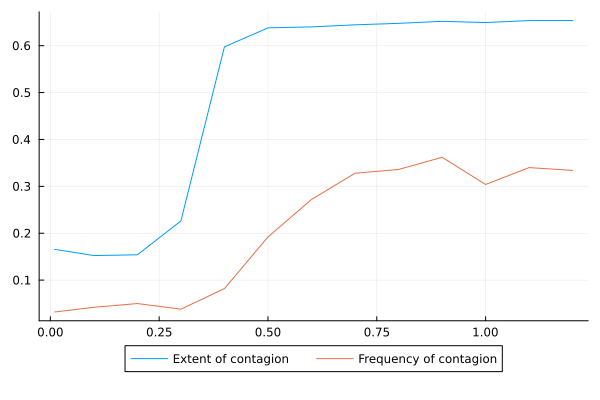
\includegraphics[scale=0.45]{contagionplot_optim.png}
  \caption{contagion for different risk aversion parameters $\gamma$}
\end{figure}

Another interesting realtion is the heterogeneity of risk aversion. When we let risk aversion parameter be random variable distributed as $\gamma_i \sim N(0.3, \sigma_{\gamma})$, then the standard deviation $\sigma_{\gamma}$ shows a heterogeneity of risk apetite among banks. Figure 3 shows the variable of interest for different values of $\sigma_{\gamma}$. 

\begin{figure}[h]
  \centering
  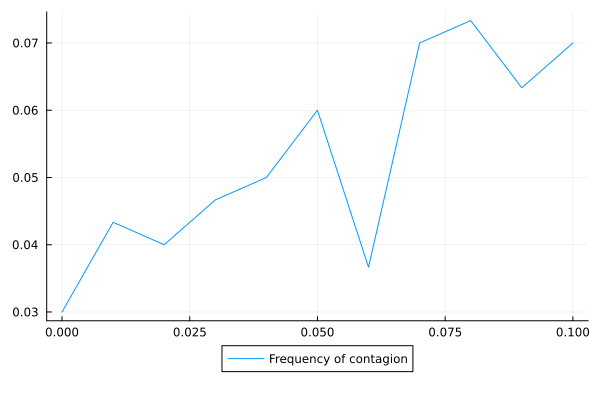
\includegraphics[scale=0.45]{contagion_freq1.png}
  \caption{contagion for different risk aversion heterogeneity among banks $\sigma_{\gamma}$}
\end{figure}

Despite having on average the same risk apetite, it is increasingly more damaging the more risk aversion varies. This is a similar phenomenon as "super-spreaders" in epidemiology, where a single entity plays a majority role in the contagion dynamics. This suggests that it is preffered from system point of view to have banks with similar risk aversion, even apart from the level of thereof.

By completing the standard model with endogenous interbank market formation we could see how the reactions of banks influence the contagion dynamics.

The code of of this section can be found on my github repository here: \url{https://github.com/m-dadej/network_contagion}

\medskip

\newpage

\bibliography{sample}

\end{document}
